\thispagestyle{toanhocvadoisongnone}
\pagestyle{toanhocvadoisong}
\everymath{\color{toanhocdoisong}}
\graphicspath{{../toanhocdoisong/pic/}}
\begingroup
\blfootnote{$^1$\color{toanhocdoisong}Viện Sinh học và Môi trường Đông Dương.}
\AddToShipoutPicture*{\put(0,616){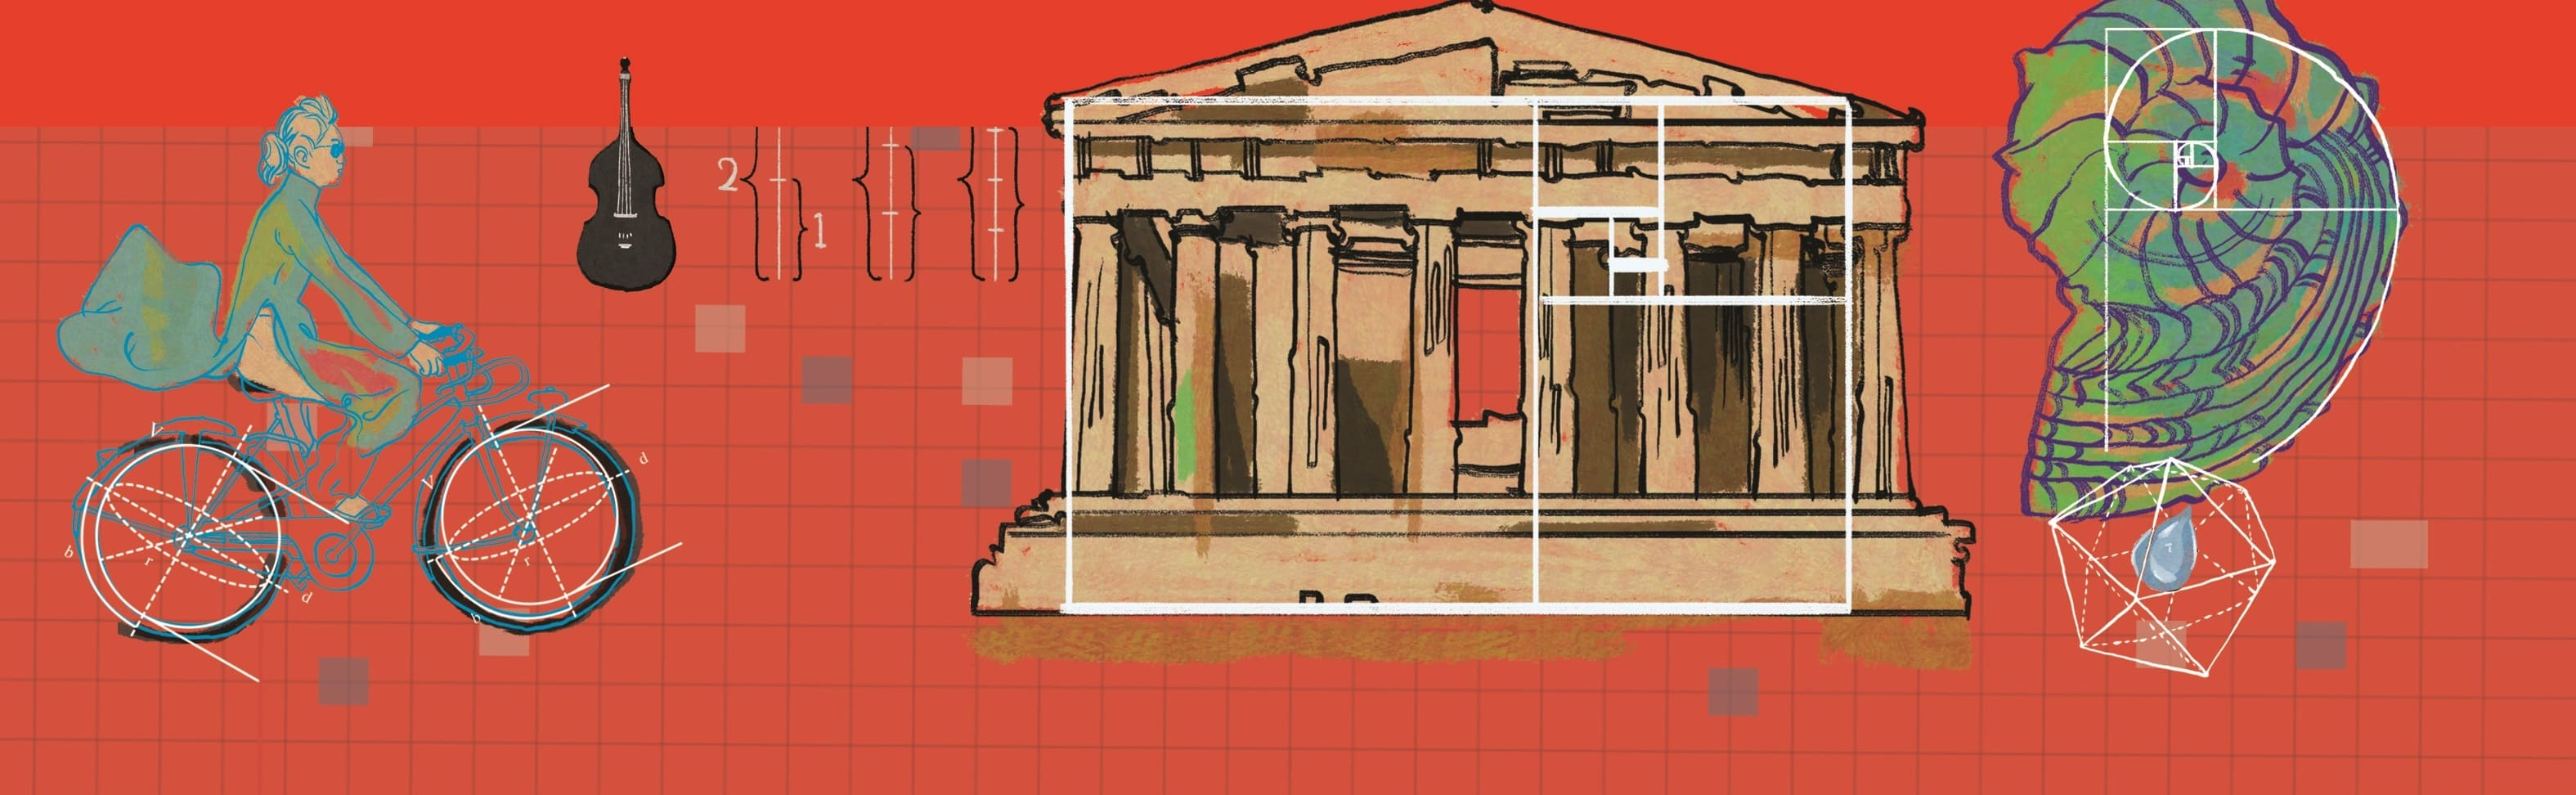
\includegraphics[width=19.3cm]{../bannertoanhocdoisong}}}
\AddToShipoutPicture*{\put(72,488){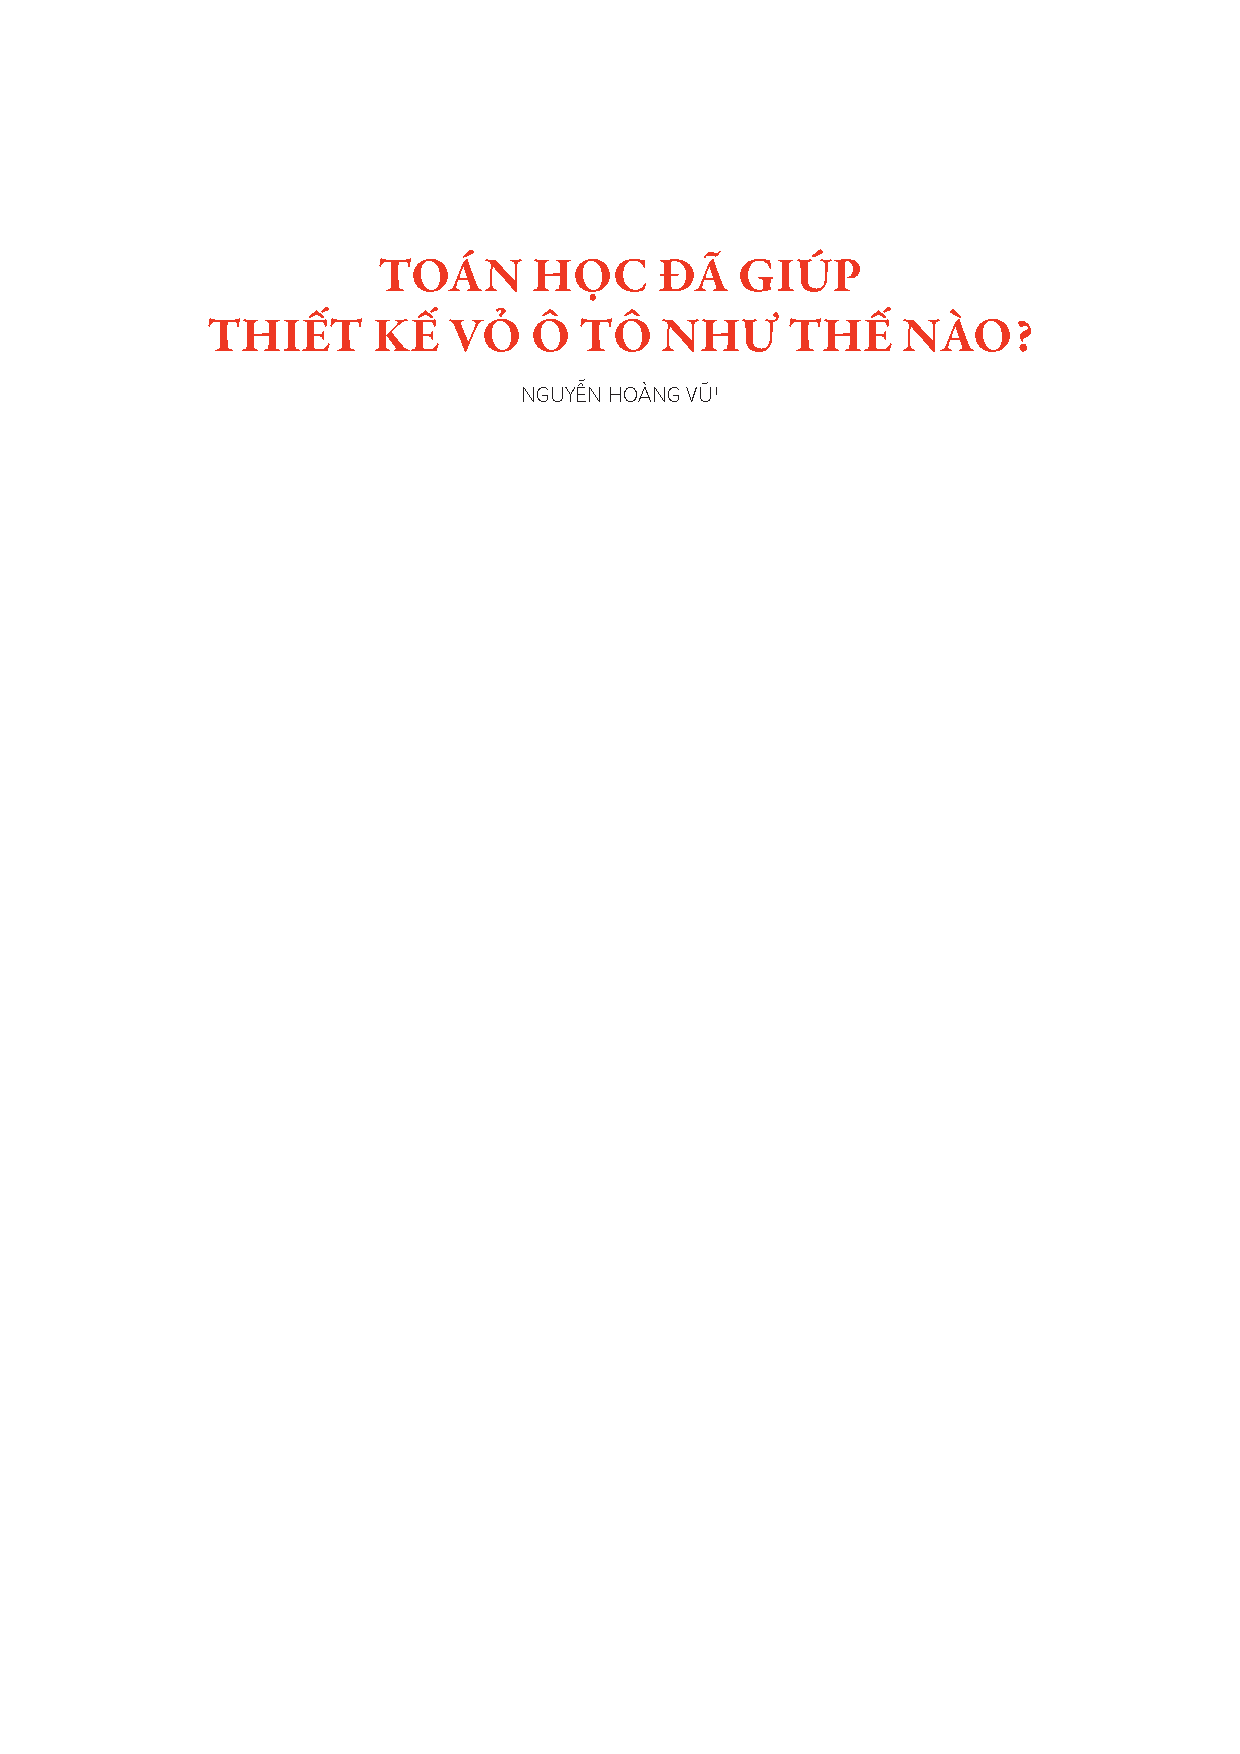
\includegraphics[scale=1]{../tieude.pdf}}}
\centering
\endgroup

\vspace*{230pt}

\textit{Origami không chỉ là một nghệ thuật gấp giấy mà còn ẩn chứa những ý nghĩa toán học sâu sắc cùng các ứng dụng bất ngờ mà chúng ta sẽ cùng tìm hiểu trong bài viết này.}
\begin{multicols}{2}
	$\pmb{1.}$ \textbf{\color{toanhocdoisong}Mở đầu}
	%	\vskip 0.1cm	
	\begin{figure}[H]
		%		\vspace*{5pt}
		\centering
		\captionsetup{labelformat= empty, justification=centering}
		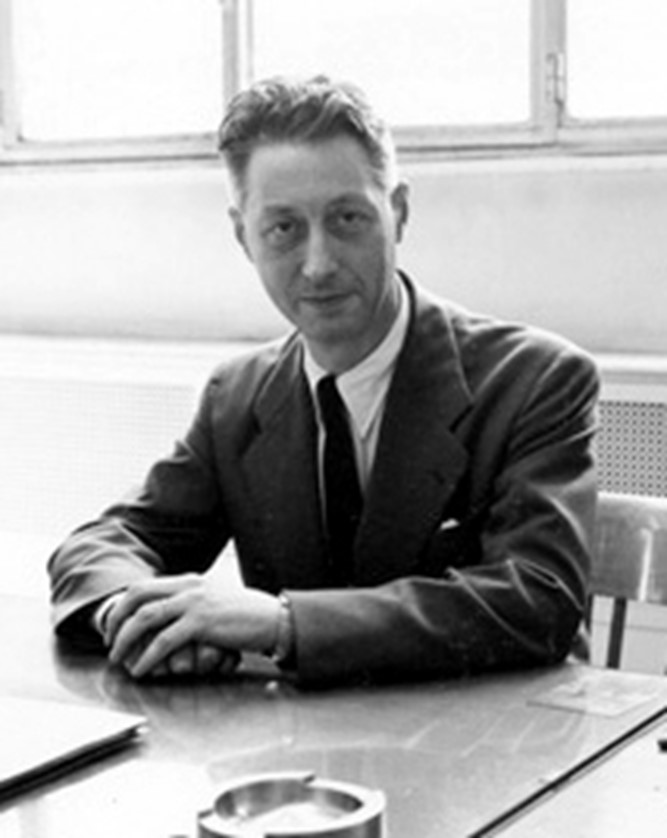
\includegraphics[height= 0.189\textwidth]{1}\hspace*{4pt}
		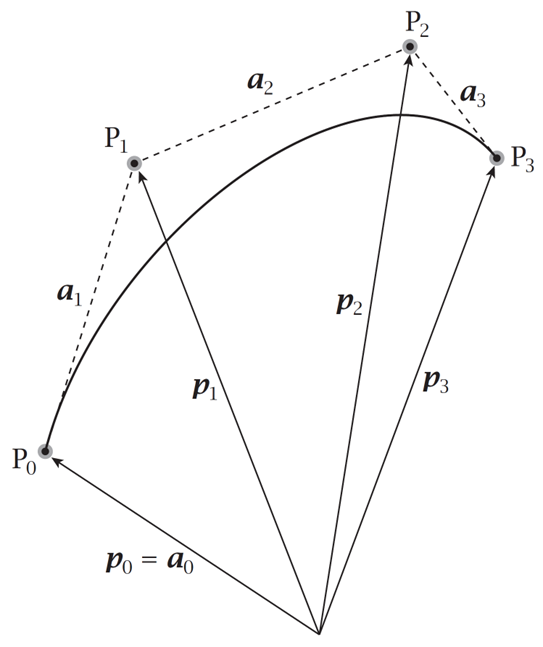
\includegraphics[height= 0.189\textwidth]{2}
		
		\vspace*{4pt}
		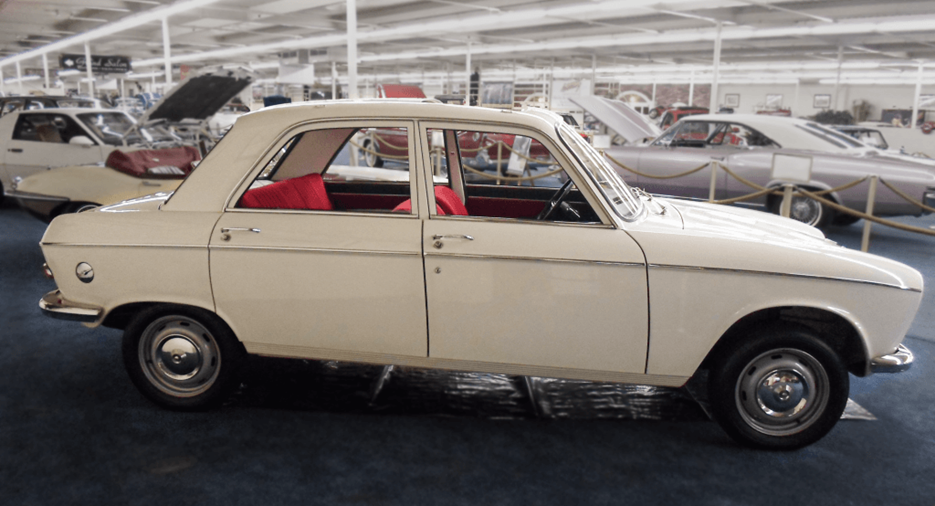
\includegraphics[width= 1\linewidth]{3}
		\caption{\small\textit{\color{toanhocdoisong}Hình $1$. Origami là nghệ thuật gấp giấy truyền thống lâu đời của Nhật Bản. Ngoài những hình gấp quen thuộc như con hạc, origami còn có thể được dùng để gấp các vật dụng thực tế, ví dụ như hộp giấy.}}
		\vspace*{-10pt}
	\end{figure}
	Origami là một trò chơi và một dạng nghệ thuật lâu đời từ nhiều thế kỷ ở Nhật Bản. Trong tiếng Nhật, \textit{ori} nghĩa là gấp còn \textit{gami} là giấy. Người gấp luôn bắt đầu từ một tờ giấy hình vuông và sau nhiều thao tác, sẽ gấp nó thành một hình theo ý muốn mà không sử dụng kéo hay hồ dán.  
	\vskip 0.1cm
	Một trong những hình origami phổ biến nhất ở Nhật Bản và trên thế giới là con hạc giấy quen thuộc. Nhiều hình gấp origami khác cũng là những hình ảnh quen thuộc trong đời sống: bông hoa, cái cây, con ngựa, các nhân vật với nghề nghiệp khác nhau, \ldots\, Có thể nói, origami phản ánh đời sống tâm hồn cùng những quan sát tinh tế về thế giới xung quanh của người Nhật Bản. Một đặc điểm của origami là dễ học và không đòi hỏi nhiều về vật liệu. Người ta có thể dùng bất cứ loại giấy nào, có thể tái sử dụng giấy báo, vỏ bao bì, \ldots\, Những hình origami cơ bản cũng không quá khó và mọi đối tượng đều có thể học được. Những người chuyên sâu hơn có thể sử dụng những loại giấy với chất liệu cao cấp và hoa văn trang trí đẹp mắt để gấp những hình phức tạp và cầu kỳ. Origami còn giúp ích cho đời sống thường ngày. Với những thao tác không quá khó, người gấp có thể tạo được những hộp, giỏ bằng giấy để mang, đựng đồ vật. 
	\vskip 0.1cm
	Ngày nay, sự kết hợp giữa toán học và origami đã cho ra đời một ngành nghiên cứu mới: origami hình học. Trong đó, người ta quan tâm đến các tính chất hình học của những cách gấp origami, đưa ra chứng minh một cách chặt chẽ, và tiến hành áp dụng các kết quả trong khoa học và kỹ thuật. 
	\vskip 0.1cm
	$\pmb{2.}$ \textbf{\color{toanhocdoisong}Bài toán gấp bản đồ}
	\vskip 0.1cm
	Ta hãy bắt đầu với một vấn đề tưởng như rất đơn giản. Nếu đã từng sử dụng bản đồ giấy mua từ cửa hàng đã được gấp sẵn một cách vuông vức, bạn có thể giở nó ra mà không có vấn đề gì nhưng việc gấp lại như ban đầu lại không dễ dàng chút nào hết.
	\vskip 0.1cm
	Tất nhiên, toán học luôn có những cách độc đáo để làm cho vấn đề trở nên bớt khó khăn hơn. Trước hết, ta tiến hành gấp chia đều chiều rộng theo các đường song song với các nếp gấp lồi và lõm xen kẽ. Sau đó, gấp theo các đường song song nhưng \textbf{\color{toanhocdoisong}không} vuông góc với cạnh hình chữ nhật như trong Hình $2$ (các hướng dẫn gấp thường yêu cầu lệch so với góc vuông khoảng $6$ độ) (Hình $2$).
	\begin{figure}[H]
		\vspace*{-5pt}
		\centering
		\captionsetup{labelformat= empty, justification=centering}
		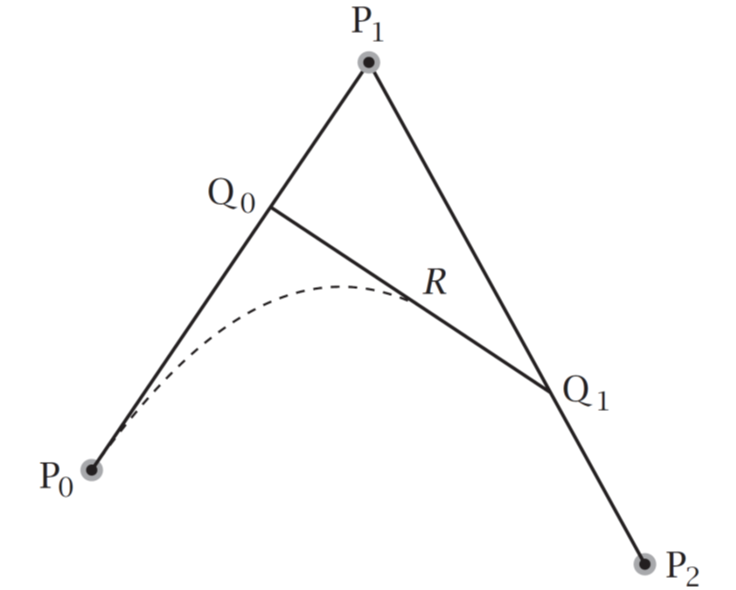
\includegraphics[width=1\linewidth]{4}
		
		\vspace*{4pt}
		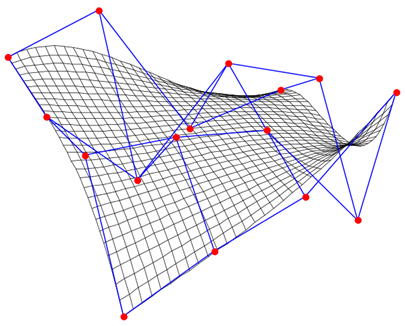
\includegraphics[width=1\linewidth]{5}
		\caption{\small\textit{\color{toanhocdoisong}Hình $2$. Các thao tác gấp bản đồ của bước $1$.}}
		\vspace*{-5pt}
	\end{figure}
	Sau khi đã có các nếp gấp, ta trải tờ giấy ra và tạo các vết hằn cho từng đoạn. Chú ý: nét liền màu xanh là nếp gấp lồi, nét đứt màu đỏ là nếp gấp lõm (Hình $3$).
	\begin{figure}[H]
		\vspace*{-5pt}
		\centering
		\captionsetup{labelformat= empty, justification=centering}
		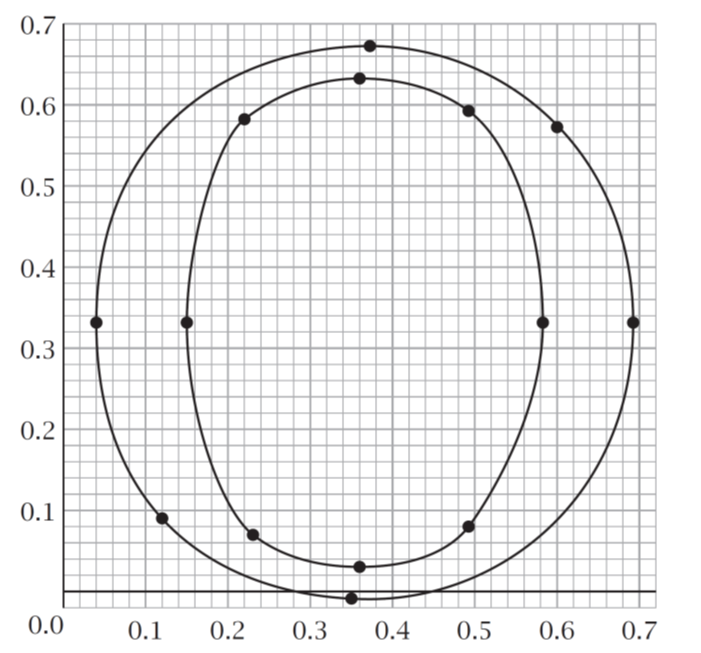
\includegraphics[height= 0.214\textwidth]{6}\hspace*{3pt}
		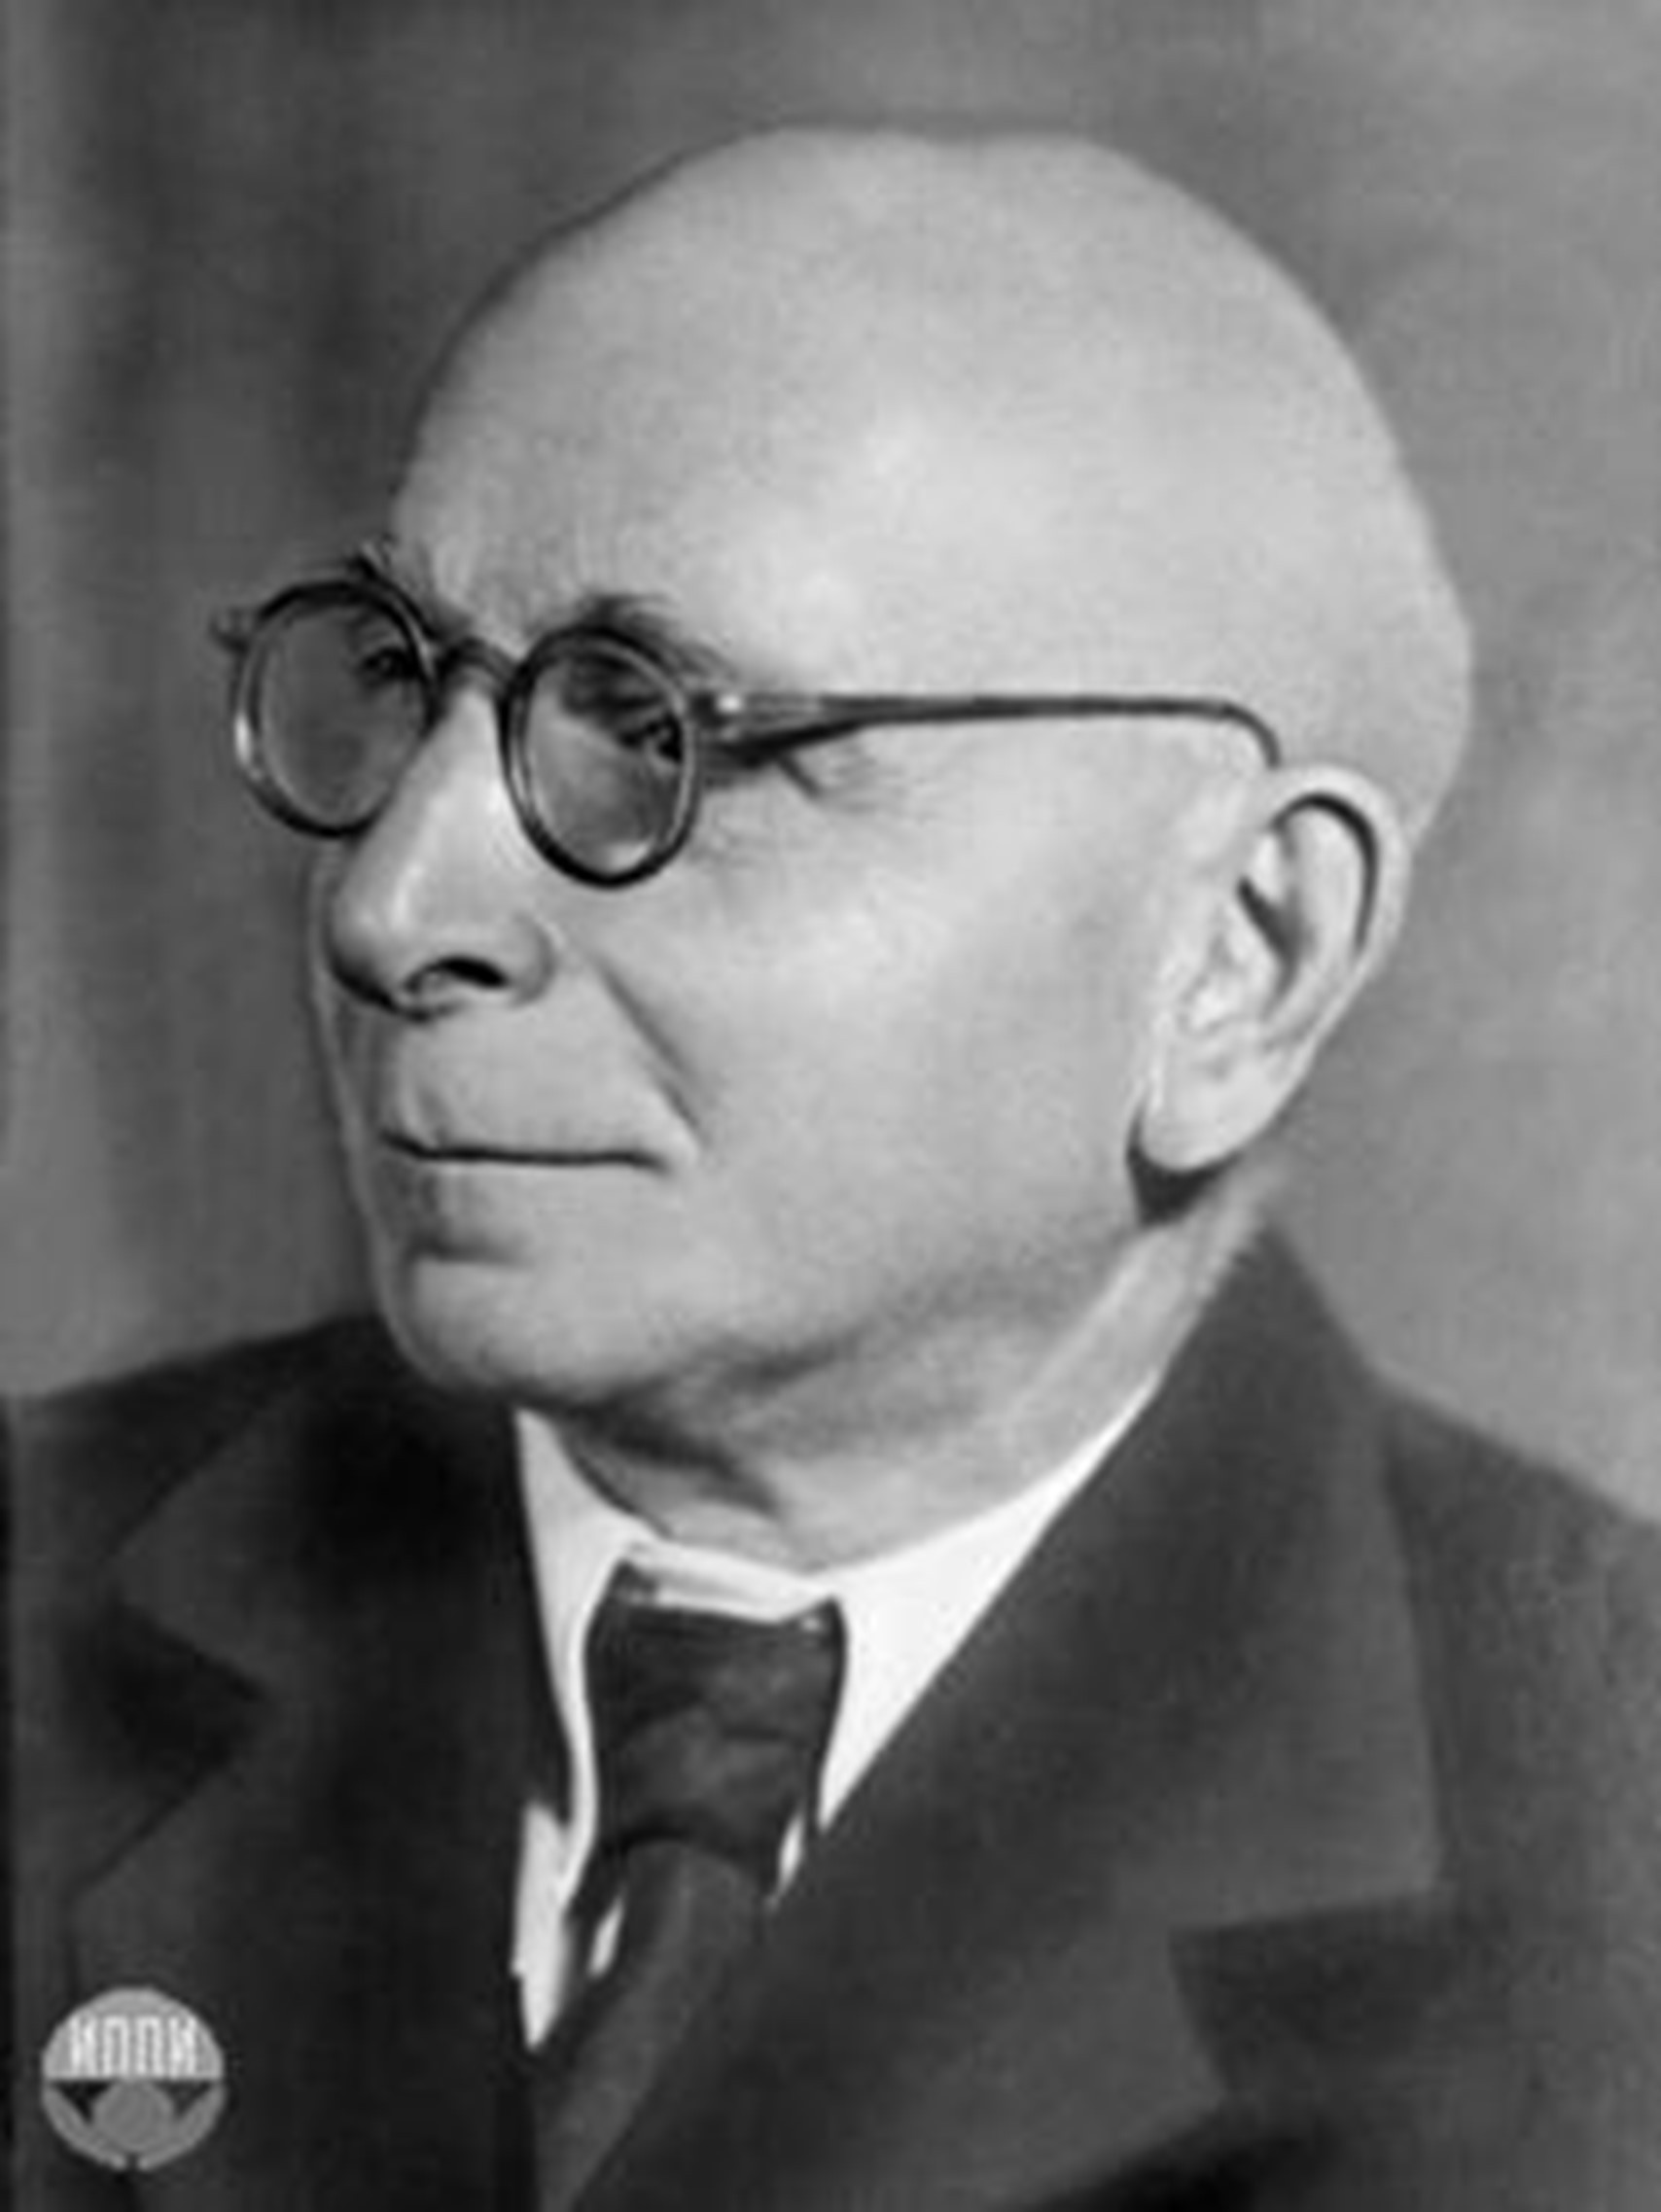
\includegraphics[height= 0.214\textwidth]{7}
		\caption{\small\textit{\color{toanhocdoisong}Hình $3$. Trải ra và hoàn thiện.}}
		\vspace*{-10pt}
	\end{figure}
	Sau khi được gấp như trên, người dùng chỉ cần cầm hai góc đối diện của bản đồ để tiến hành mở ra hoặc gấp vào một cách dễ dàng (Hình $4$). 
	\begin{figure}[H]
		\vspace*{-5pt}
		\centering
		\captionsetup{labelformat= empty, justification=centering}
		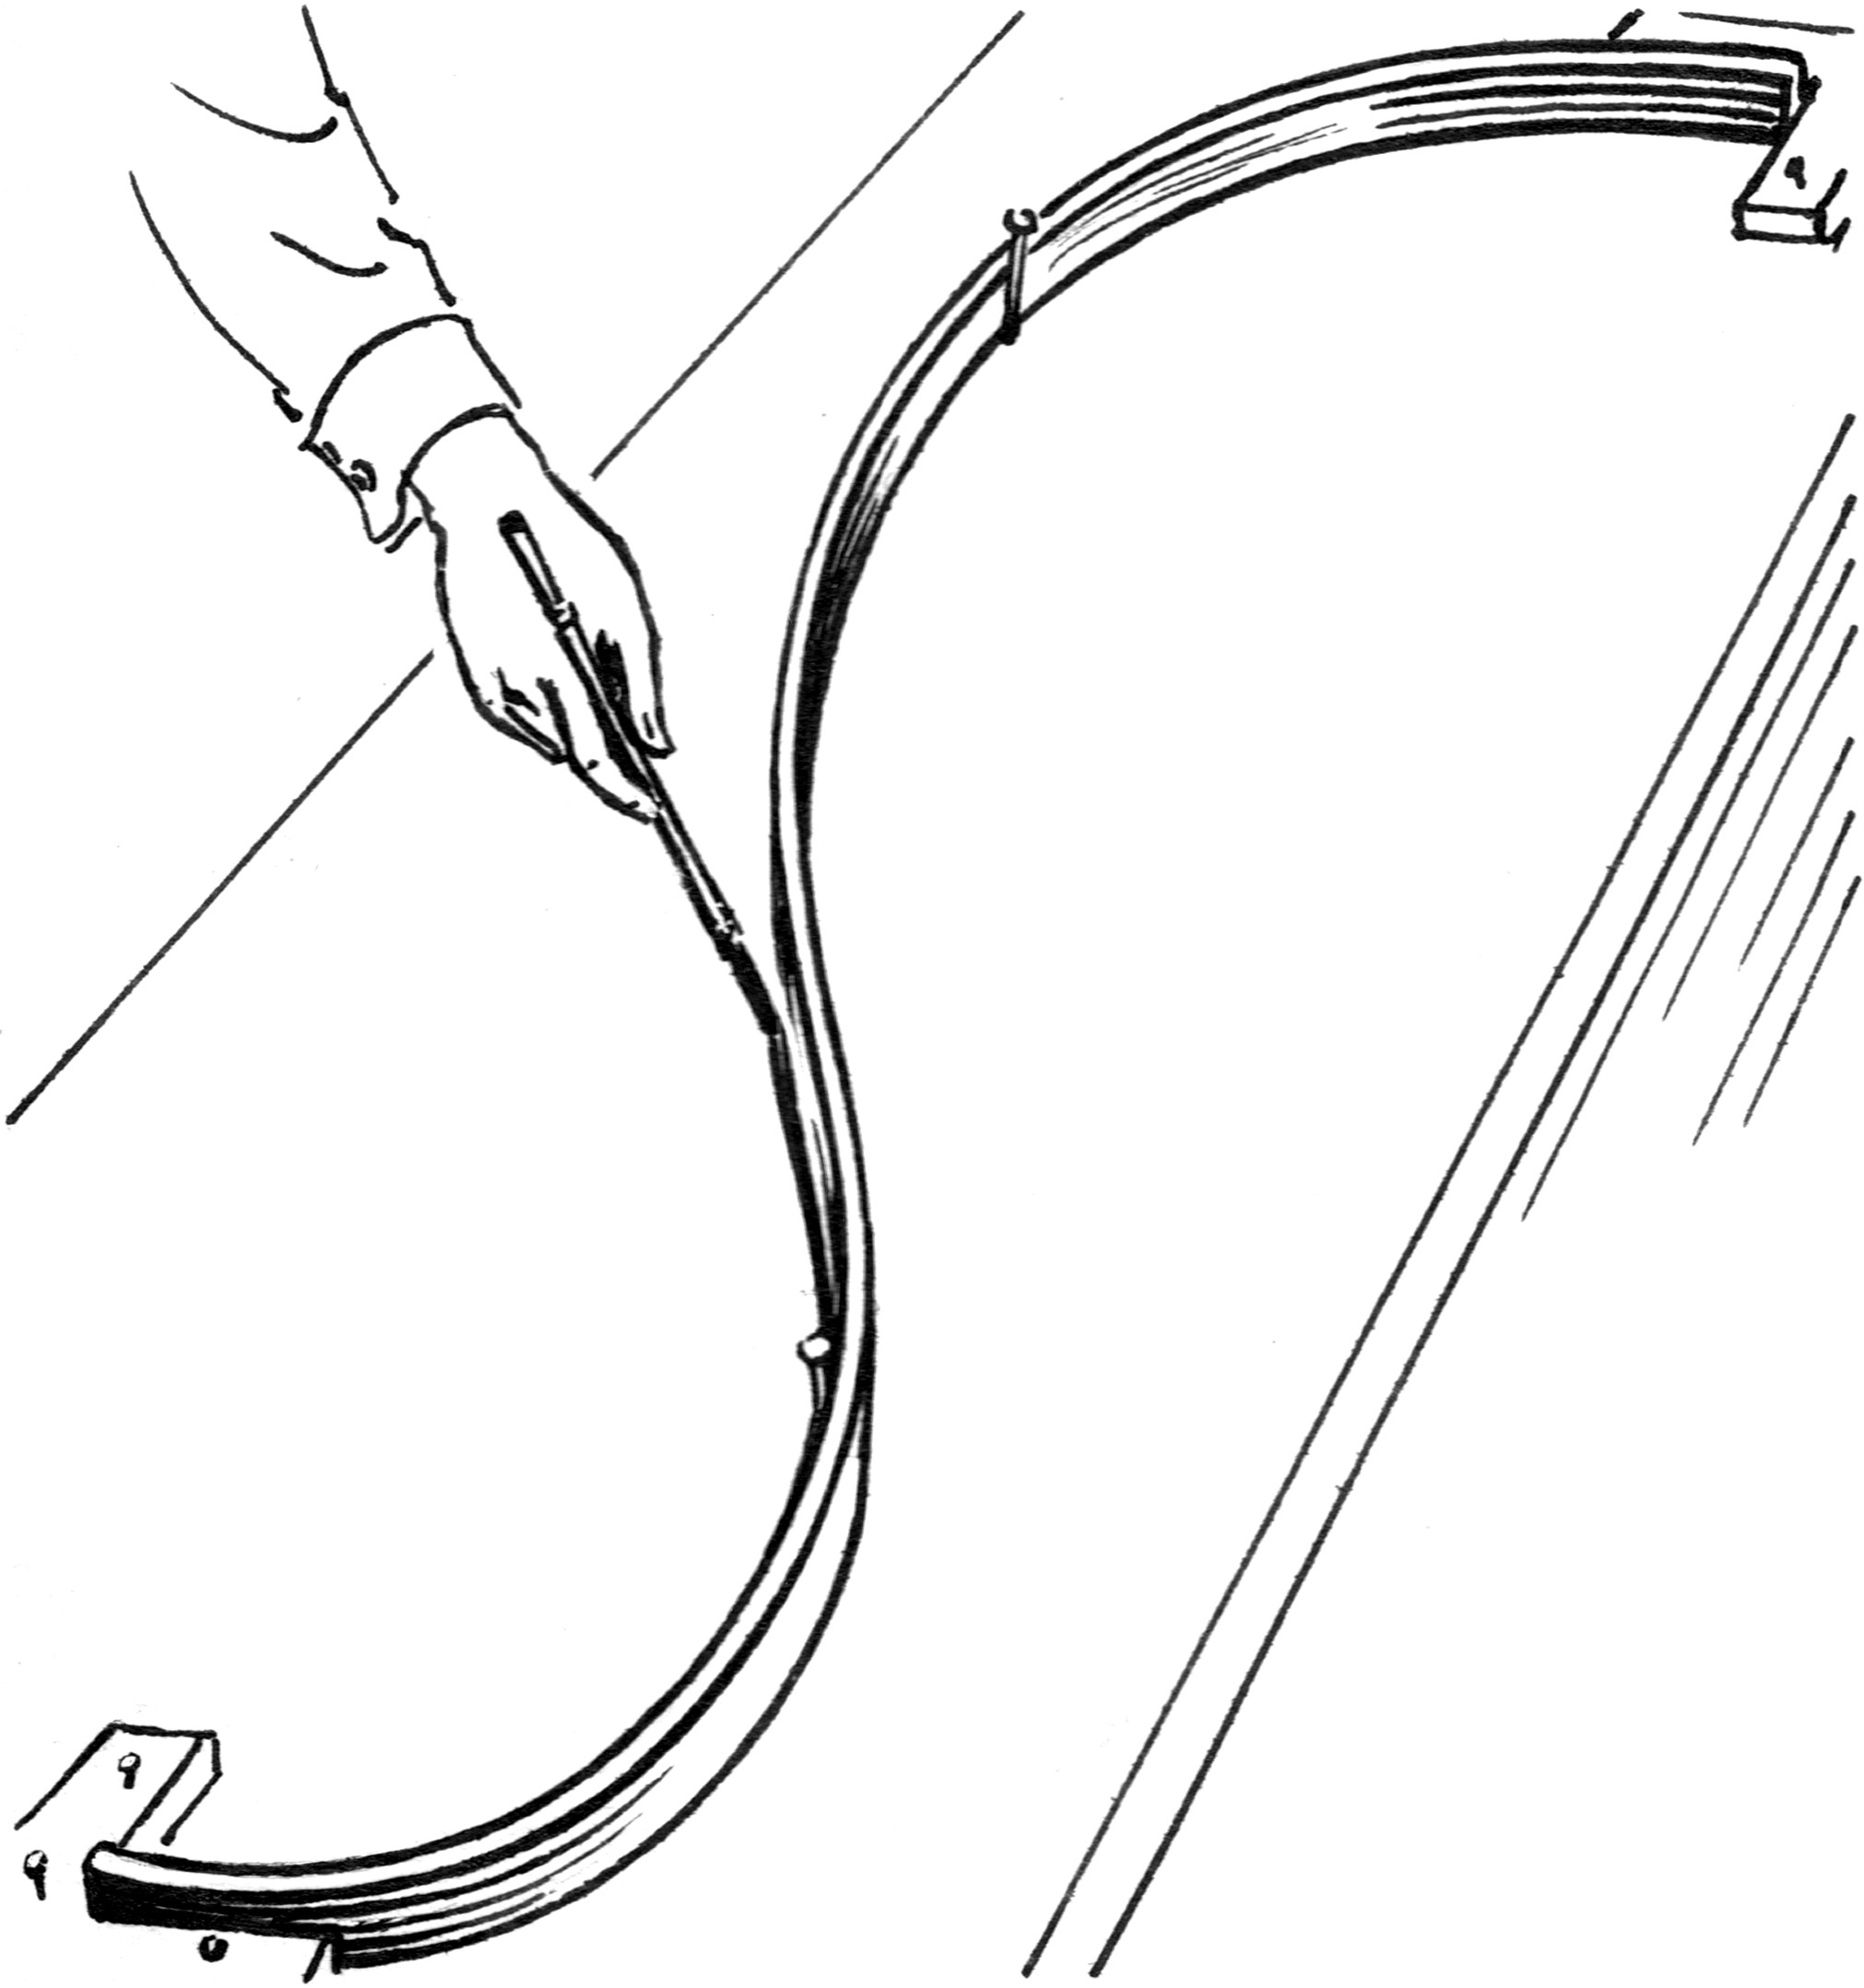
\includegraphics[width=1\linewidth]{8}
		\caption{\small\textit{\color{toanhocdoisong}Hình $4$. Thao tác với bản đồ sau khi gấp.}}
		\vspace*{-10pt}
	\end{figure}
	$\pmb{3.}$ \textbf{\color{toanhocdoisong}Miura--ori}
	\vskip 0.1cm
	Cách gấp bản đồ trên được đề xuất bởi nhà vật lý thiên văn người Nhật tên là Koryo Miura. Do đó, nó còn được gọi là Miura--ori (theo tiếng Nhật, nghĩa là nếp gấp Miura).
	\vskip 0.1cm
	Nếp gấp của Miura bắt nguồn từ các công trình nghiên cứu của Yoshimura. Yoshimura\linebreak nhận thấy một hiện tượng của các bề mặt hình trụ, ví dụ như vỏ lon nước ngọt: khi chịu tác động cơ học, bề mặt  hình trụ có thể xuất hiện một mạng hình thoi, ngày nay còn được gọi là mẫu Yoshimura (Yoshimura pattern). Điều đáng chú ý là quá trình này giống với gấp giấy origami: bề mặt bị gấp nhưng không bị kéo dãn (tổng diện tích bề mặt không đổi). Những biến đổi này có thể xảy ra với năng lượng tác động rất ít và không lường trước, nên có thể rất nguy hiểm khi nó xảy ra.
	\vskip 0.1cm
	Miura đã đặt câu hỏi liệu có một hiện tượng tương tự với các cấu trục phẳng và mỏng, có thể coi là $2$ chiều hay không. Trong bài báo năm $1970$, ông đã đề xuất một bề mặt được tạo ra từ các nếp gấp origami. Giả thuyết này sau đó đã được kiểm chứng bằng cả tính toán và thực nghiệm.
	\begin{figure}[H]
		\vspace*{-5pt}
		\centering
		\captionsetup{labelformat= empty, justification=centering}
		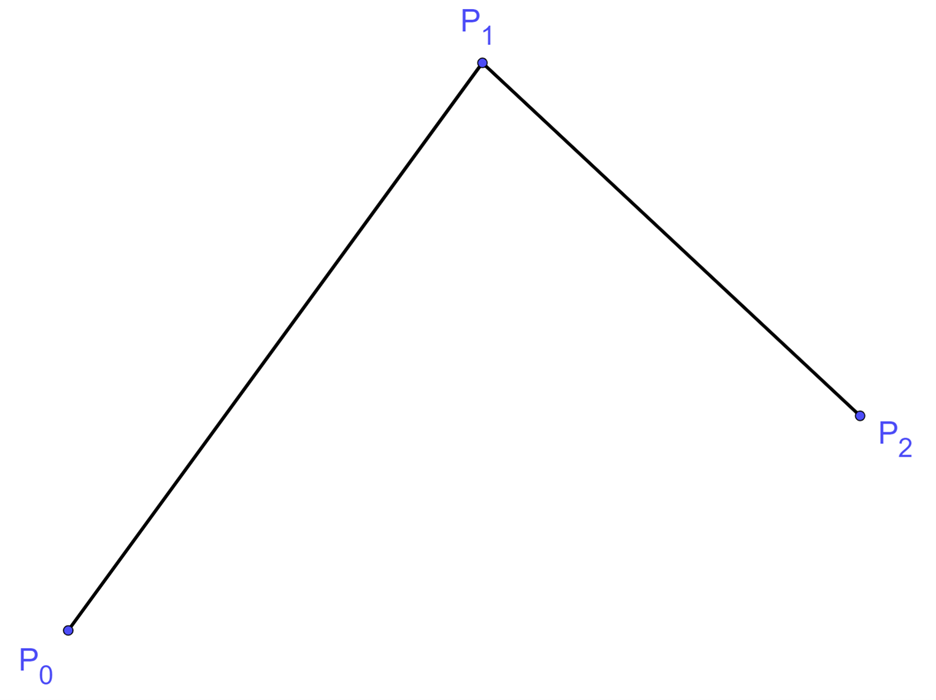
\includegraphics[width= 1\linewidth]{9}
		
		\vspace*{4pt}
		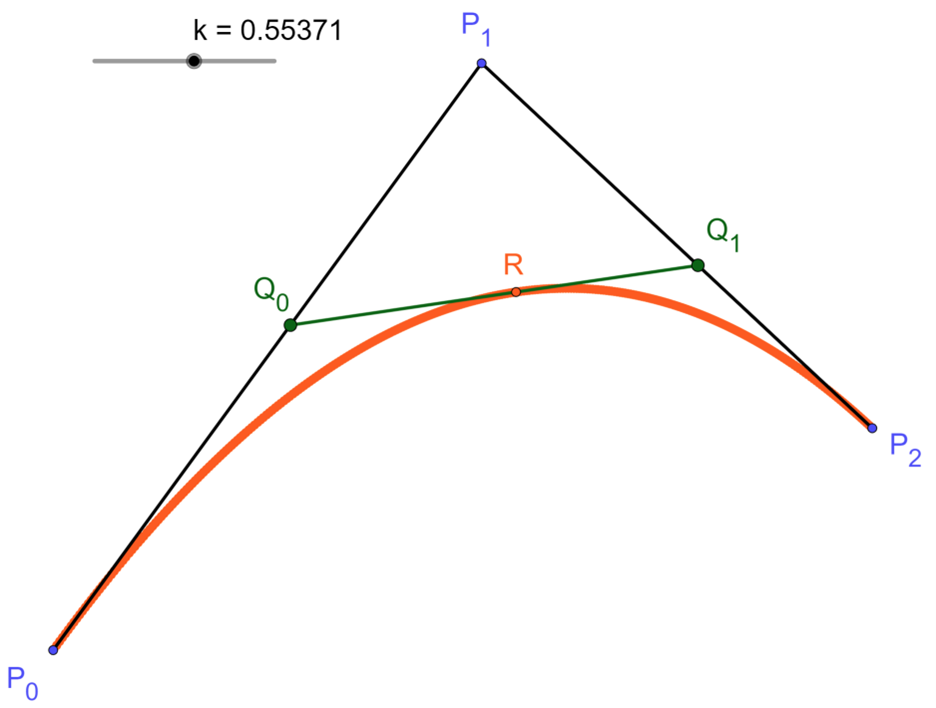
\includegraphics[height= 0.21\textwidth]{10}\hspace*{3pt}
		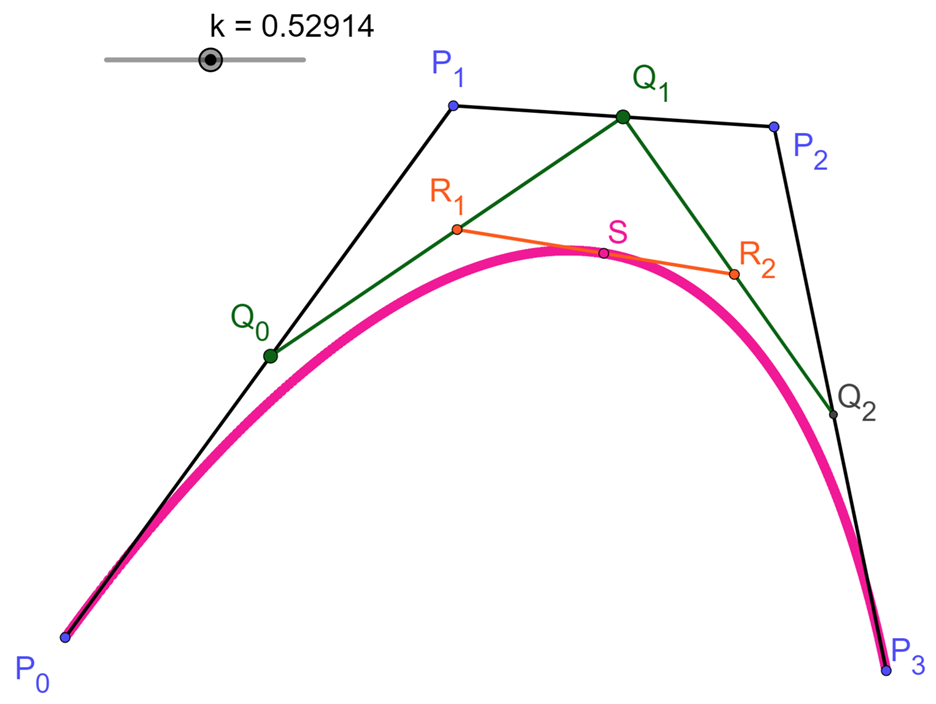
\includegraphics[height= 0.21\textwidth]{11}
		\caption{\small\textit{\color{toanhocdoisong}Hình $5$. Mẫu Yoshimura khi trải phẳng. Hiện tượng Yoshimura quan sát thấy trên bề mặt hình trụ (dưới, bên trái). Tay áo của nàng Mona Lisa trong tranh của Leonardo da Vinci cũng có những nếp nhăn tương tự (dưới, bên phải).}}
		\vspace*{-10pt}
	\end{figure}
	Các nếp gấp mà dọc theo chiều của nó, tất cả các nếp gấp đều cùng lồi hoặc cùng lõm được gọi là các nếp gấp chính. Các nếp gấp còn lại được gọi là các nếp gấp phụ. Miura--ori có thể coi là một họ các nếp gấp với các tham số thay đổi bao gồm: độ dài nếp gấp chính $d_1$, độ dài nếp gấp phụ $d_2$ và góc $\alpha$ giữa nếp gấp chính và phụ. 
	
	\begin{figure}[H]
		\vspace*{-5pt}
		\centering
		\captionsetup{labelformat= empty, justification=centering}
		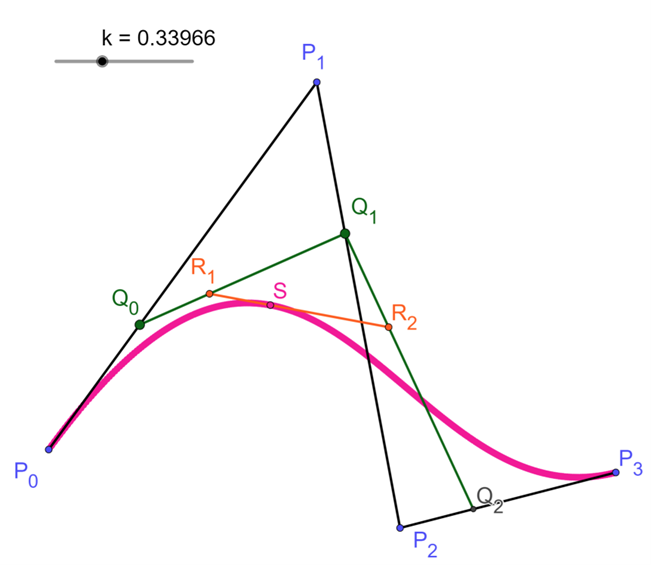
\includegraphics[height= 0.21\textwidth]{12}
		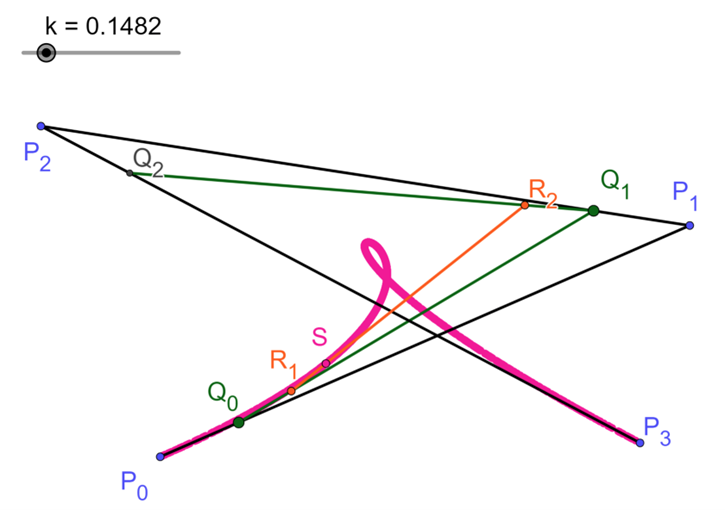
\includegraphics[height= 0.21\textwidth]{13}
		\caption{\small\textit{\color{toanhocdoisong}Hình $6$. Koryo Miura trình diễn về mô hình của mình (bên trái). Nếp gấp Miura với các tham số (phải). Nét liền là nếp gấp lồi, nét đứt là nếp gấp lõm (tất cả các hình minh họa sau này đều theo quy tắc này).}}
		\vspace*{-5pt}
	\end{figure}
	Điều đáng chú ý là khi $\alpha =90^\circ$ thì các mặt hình bình hành trở thành hình chữ nhật nhưng chuyển động của các nếp gấp chính và nếp gấp phụ bị hoàn toàn tách biệt với nhau trong quá trình kéo/đẩy và Miura--ori bị mất đi đặc tính ưu việt của nó.
	
	Về mặt lịch sử, Koryo Miura không phải là người đầu tiên đưa ra nếp gấp này. Cuốn sách dạy gấp khăn tay của Mattia Giegher năm $1639$ cũng có cách gấp tương tự. Giegher đã dạy những kỹ thuật gấp này khi ở đại học Padua (Italy ngày nay). Một bằng sáng chế về cách uốn vật liệu kim loại của Henry Hochfeld năm $1959$ cũng có cách gấp \linebreak tương tự.
	\begin{figure}[H]
		\vspace*{-5pt}
		\centering
		\captionsetup{labelformat= empty, justification=centering}
		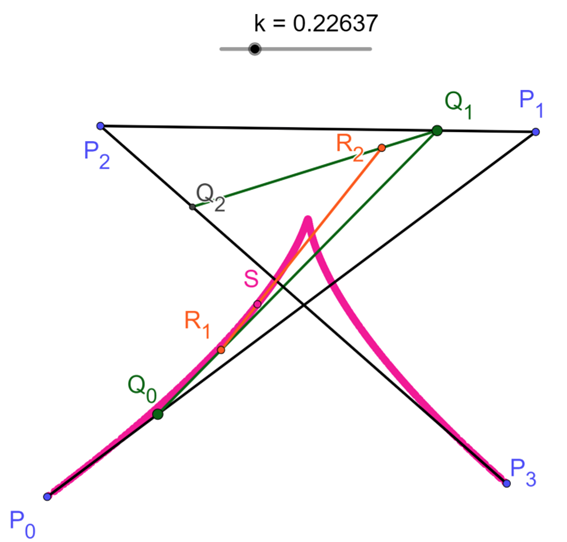
\includegraphics[width= 1\linewidth]{14}
		\caption{\small\textit{\color{toanhocdoisong}Hình $7$. Minh họa các gấp của Mattia Giegher năm $1639$, giống với Miura--ori.}}
		\vspace*{-10pt}
	\end{figure}
	\begin{figure}[H]
		\vspace*{-5pt}
		\centering
		\captionsetup{labelformat= empty, justification=centering}
		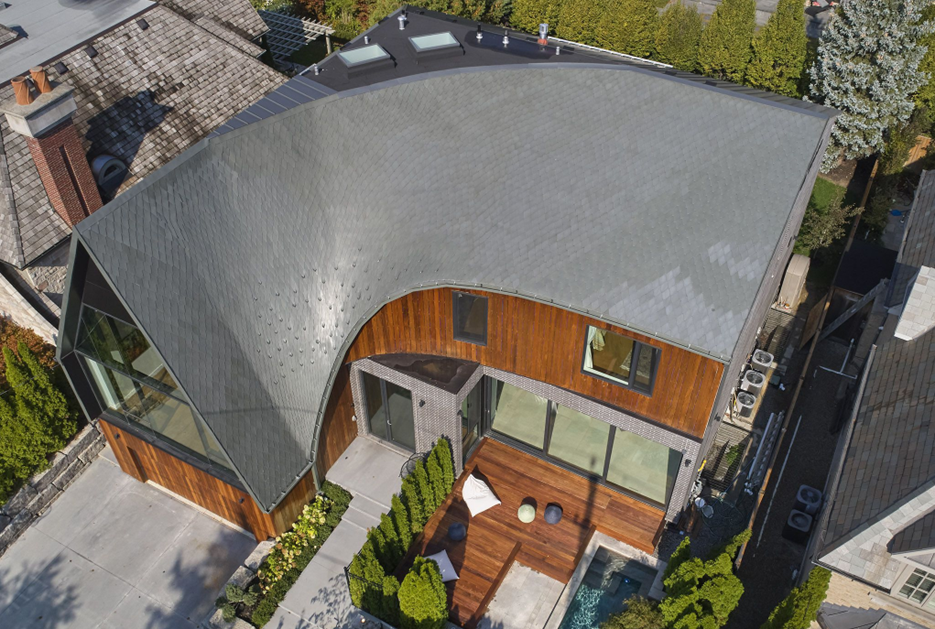
\includegraphics[width= 1\linewidth]{15}
		\caption{\small\textit{\color{toanhocdoisong}Hình $8$. Hình ảnh từ bằng sáng chế năm $1959$ của Henry Hochfield, với một phiên bản của Miura--ori.}}
		\vspace*{-10pt}
	\end{figure}
	Tuy vậy, việc nếp gấp được đặt tên theo Miura là hoàn toàn xứng đáng bởi ông là người đã tổng quát hóa và tiến hành các nghiên cứu về toán học cũng như ứng dụng nó trong \linebreak thực tế.
	\vskip 0.1cm
	Không chỉ để gấp bản đồ, Miura--ori có tác dụng lớn trong việc gấp và đóng gói nhiều loại hàng hóa khác nhau. Đặc biệt, năm $1980$, Miura, bản thân là một nhà vật lý thiên văn, đã đề xuất việc gấp các tấm pin mặt trời của vệ tinh để tiết kiệm thể tích khi phóng lên vũ trụ. Khi đã vào quỹ đạo, tấm pin sẽ được mở ra nhờ cần gạt một cách dễ dàng, tương tự như ta đã thấy với bản đồ. Năm $1995$, một vệ tinh đã được phóng lên quỹ đạo mang theo pin mặt trời được gấp theo thiết kế này và quá trình đã được tiến hành thành công.
	\begin{figure}[H]
		\vspace*{-5pt}
		\centering
		\captionsetup{labelformat= empty, justification=centering}
		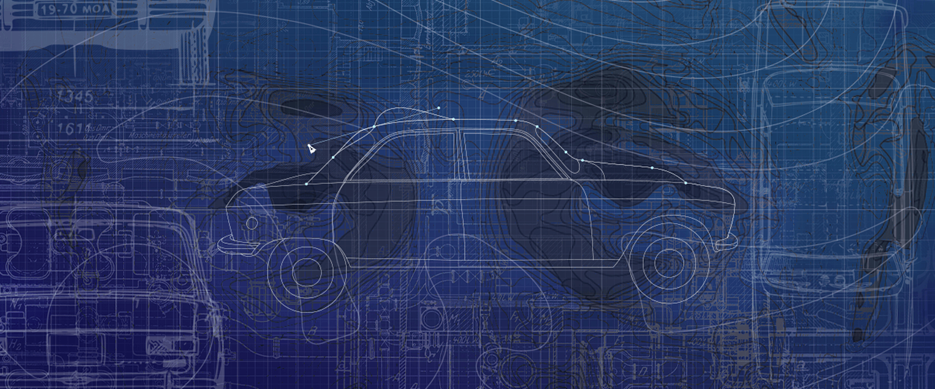
\includegraphics[width= 1\linewidth]{16}
		\caption{\small\textit{\color{toanhocdoisong}Hình $9$. Nếp gấp Miura cho pin mặt trời của vệ tinh trên vệ tinh của Nhật Bản.}}
		\vspace*{-10pt}
	\end{figure}
	Miura--ori còn xuất hiện trong nhiều sản phẩm công nghệ khác nhau. Nhóm nghiên cứu của Yves Klett tại đại học Stuttgart khi chế tạo tấm nhựa chịu lực đã sử dụng nếp gấp này thay cho cấu trúc tổ ong truyền thống với máy gấp tự động. Phiên bản này cũng được chỉnh sửa để không bị gấp lại thành dạng dẹt. Cấu trúc dạng này có khả năng chịu lực rất lớn, ví dụ như trọng lượng của một ô tô.
	\vskip 0.1cm
	Một số nghiên cứu cũng cho thấy ở một số loài cây, lá cây được cấu trúc tương tự như Miura--ori. Theo đó, quá trình lớn lên dần của của lá cây từ khi còn là búp đến khi trưởng thành cũng tương tự như quá trình bung ra của nếp gấp.  
	\begin{figure}[H]
		\vspace*{-5pt}
		\centering
		\captionsetup{labelformat= empty, justification=centering}
		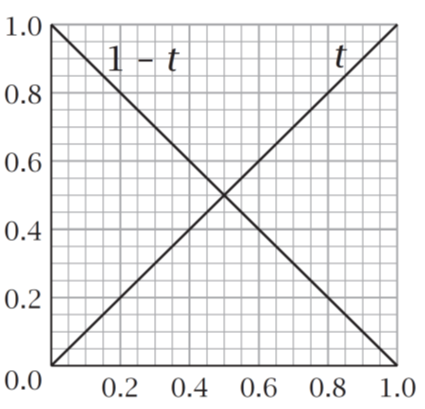
\includegraphics[width= 1\linewidth]{17}
		\caption{\small\textit{\color{toanhocdoisong}Hình $10$. Miếng nhựa chịu lực với thiết kế sử dụng Miura--ori.}}
		\vspace*{-5pt}
	\end{figure}
	\begin{figure}[H]
		\vspace*{5pt}
		\centering
		\captionsetup{labelformat= empty, justification=centering}
		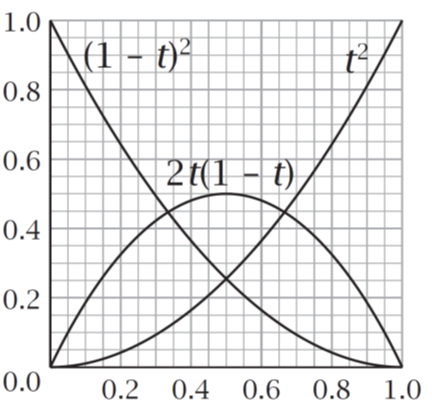
\includegraphics[width= 1\linewidth]{18}
		\caption{\small\textit{\color{toanhocdoisong}Hình $11$. Quá trình sinh trưởng của lá cây của Carpinus Betulus có sự tương đồng với nếp gấp Miura.}}
		\vspace*{-10pt}
	\end{figure}
	$\pmb{4.}$ \textbf{\color{toanhocdoisong}Một số cách gấp khác}
	\vskip 0.1cm
	Miura--ori không phải là nếp gấp duy nhất với những đặc tính thú vị. Trong origami \linebreak hình học, nhiều cách gấp khác nhau đã được nghiên cứu với các ứng dụng trực tiếp trong thực tiễn. 
	\vskip 0.1cm
	Những mẫu có sẵn có thể kết hợp với nhau để cho ra các tính chất mới. Chẳng hạn, Miura--ori và mẫu Yoshimura có đặc tính khác nhau khi bị tác động nên khi ghép chúng vào cùng một thiết kế, người ta có thể thu được những cấu trúc với trạng thái mong muốn khi bị tác động (Hình $12$).
	\begin{figure}[H]
		\vspace*{-5pt}
		\centering
		\captionsetup{labelformat= empty, justification=centering}
		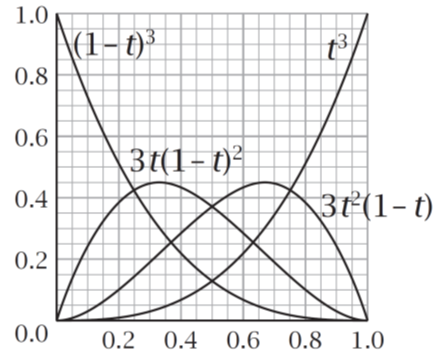
\includegraphics[width= 1\linewidth]{19}
		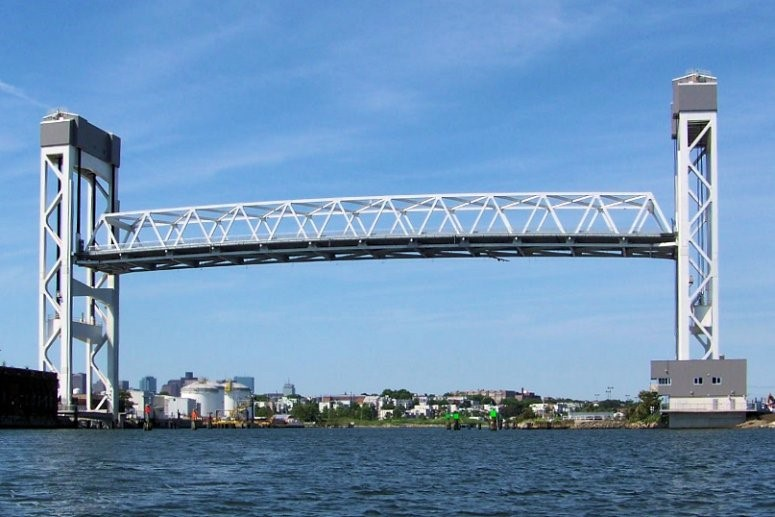
\includegraphics[width= 1\linewidth]{20}
		\caption{\small\textit{\color{toanhocdoisong}Hình $12$. Một thiết kế hỗn hợp dạng Miura-Yoshimura và trạng thái khi gấp của nó.}}
		\vspace*{-10pt}
	\end{figure}
	Trong khi mẫu Yoshimura được tạo ra khi \linebreak hình bị nén, một cách gấp khác cũng xuất hiện khi xoắn hình trụ. Các cấu trúc  này thường sẽ có hai trạng thái ổn định với chiều cao khác nhau. Người ta cũng đã nghiên cứu chế tạo ăng--ten có thể thu gọn theo cách gấp này (Hình $13$).
	\begin{figure}[H]
		\vspace*{5pt}
		\centering
		\captionsetup{labelformat= empty, justification=centering}
		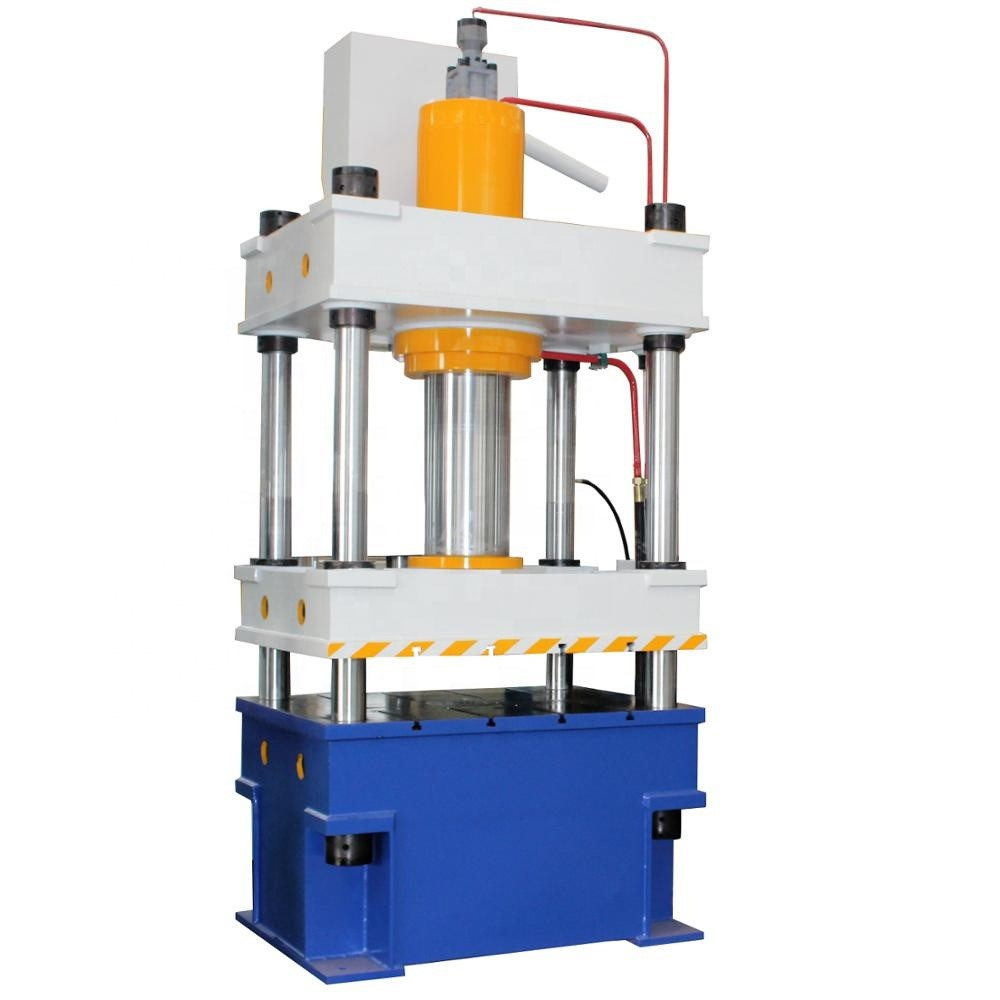
\includegraphics[height= 0.44\linewidth]{21}
		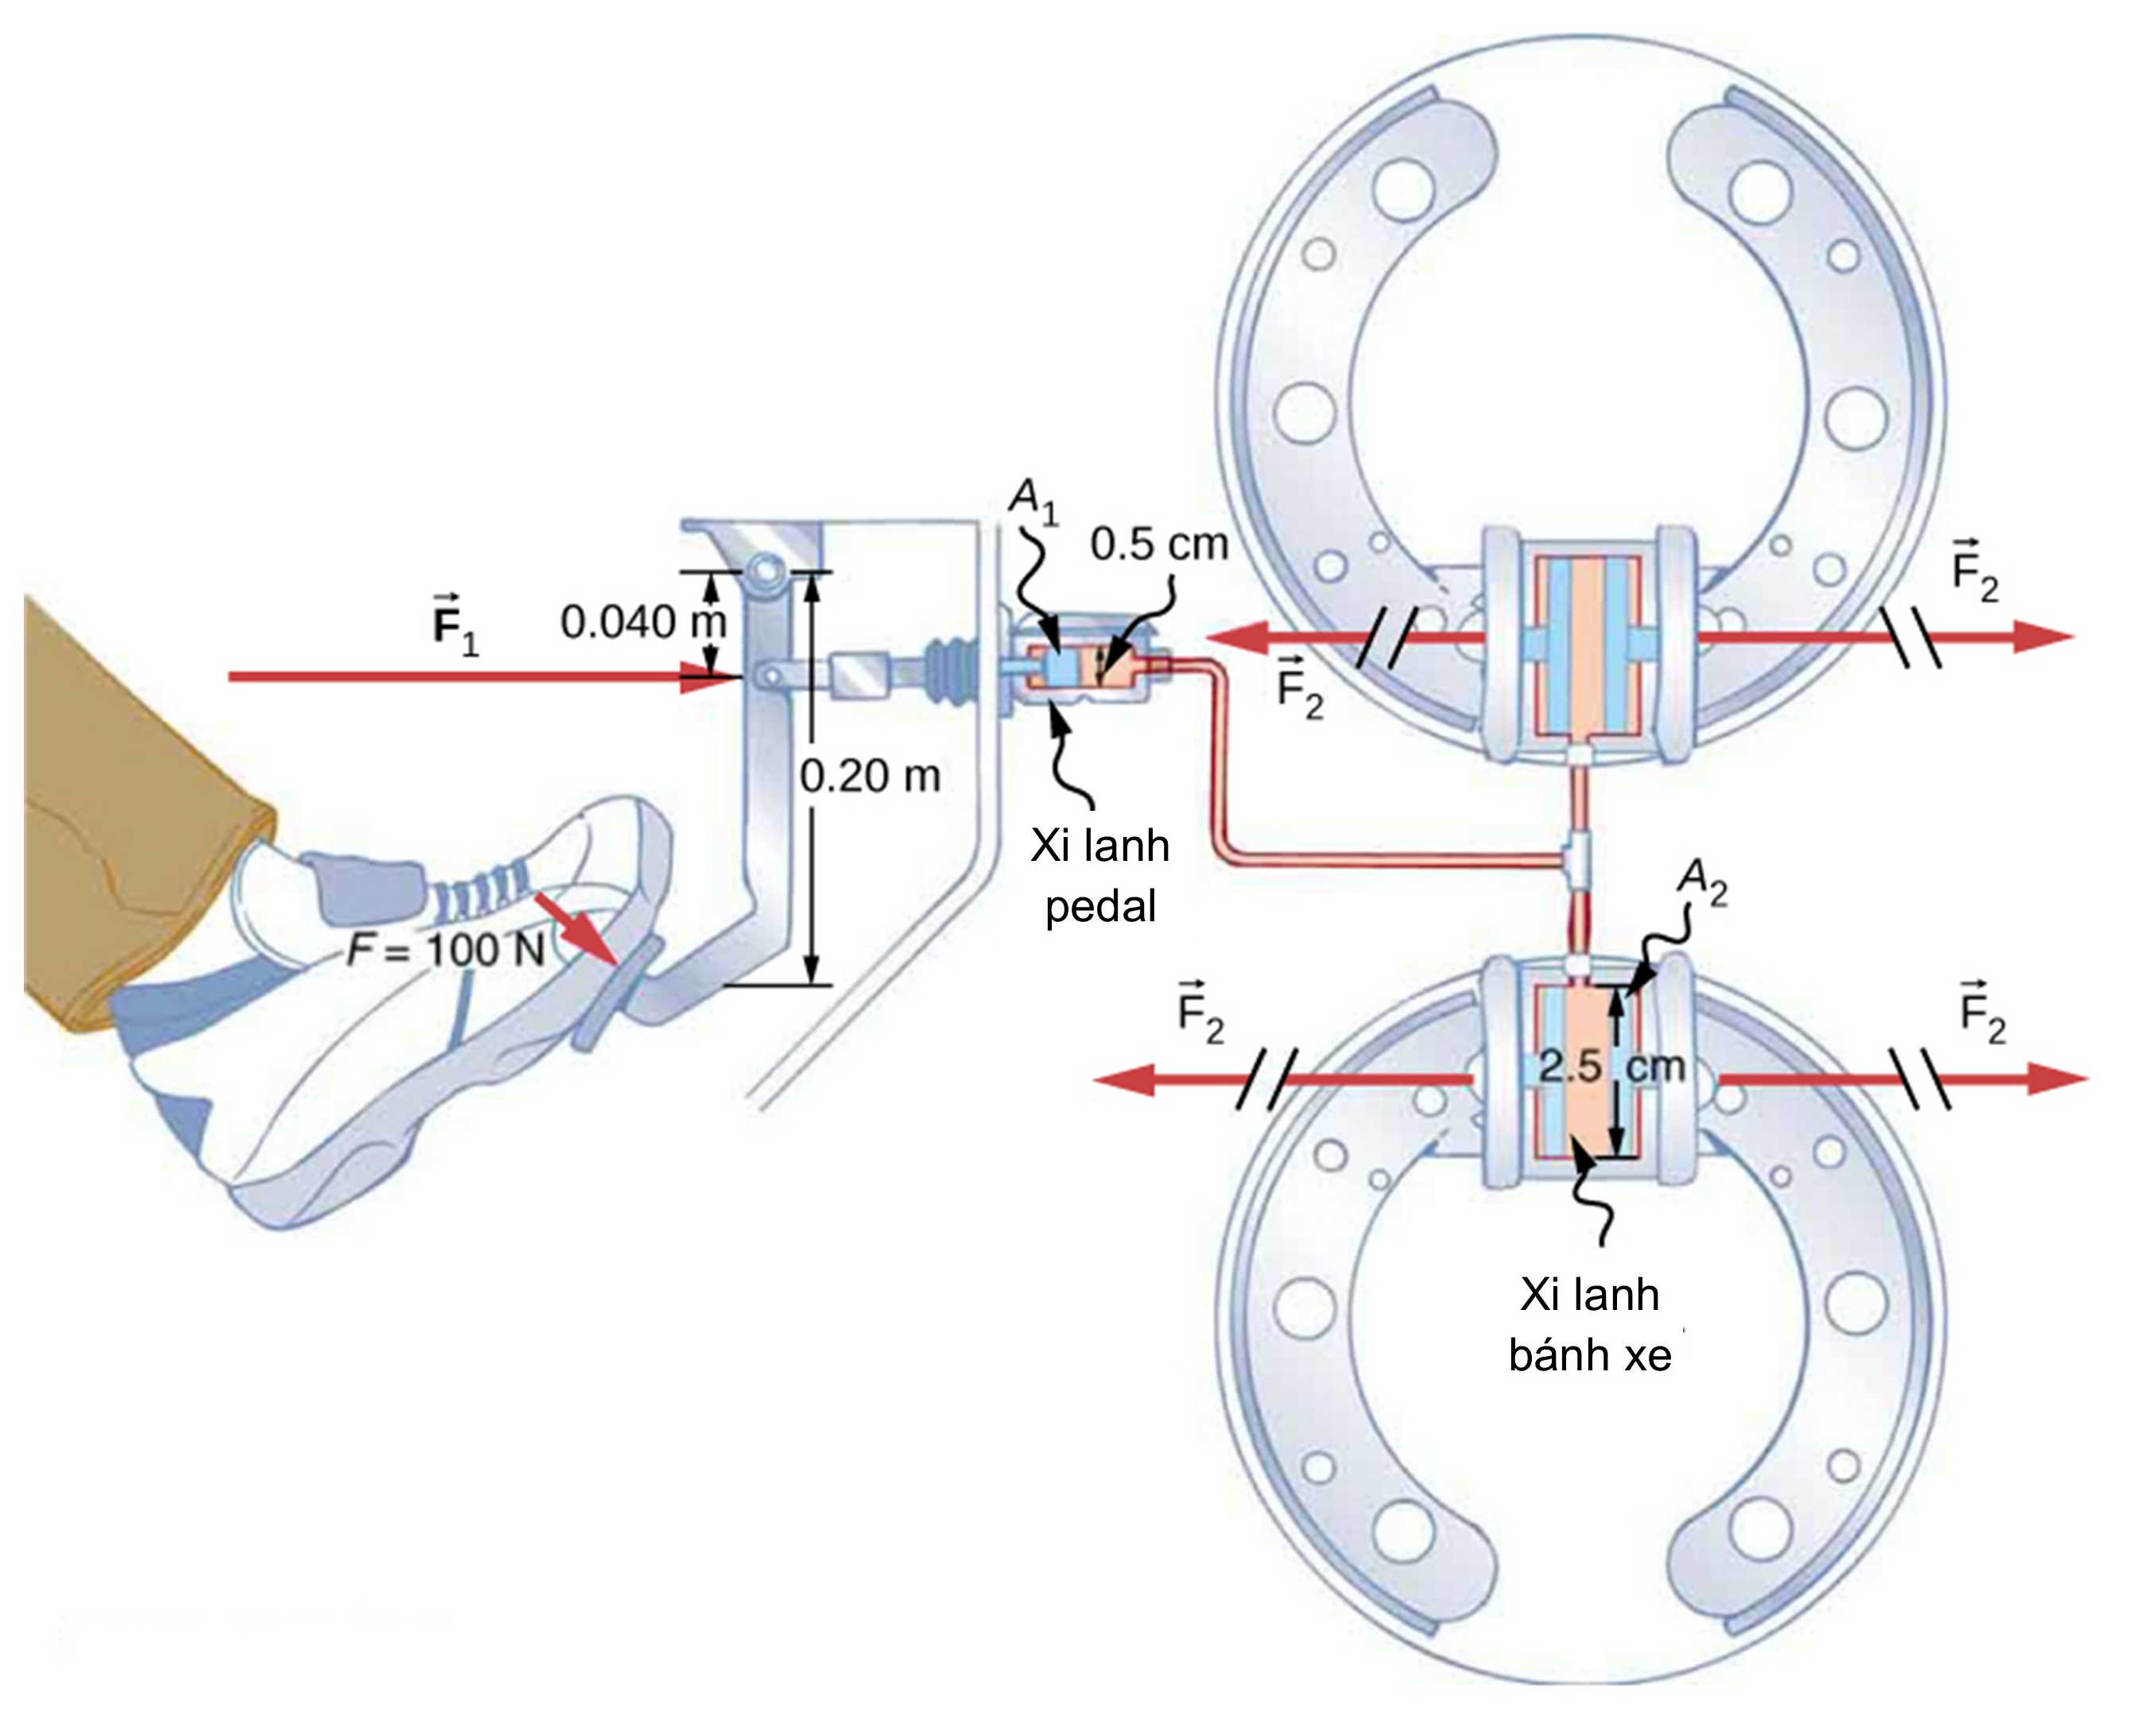
\includegraphics[height= 0.44\linewidth]{23}
		
		\vspace*{4pt}
		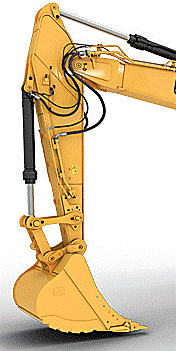
\includegraphics[width= 1\linewidth]{22}
		\caption{\small\textit{\color{toanhocdoisong}Hình $13$. Lon nước ngọt bị xoắn sẽ xuất hiện các hình tam giác trên bề mặt (bên dưới). Một ví dụ về dạng trụ xoắn với hai trạng thái ổn định (trên, bên phải). Một thiết kế ăng--ten origami dựa trên dạng hình trụ bị vặn (trên, bên trái).}}
		\vspace*{-10pt}
	\end{figure}
	Một ví dụ phức tạp hơn là thiết kế ``bom nước" (water bomb, đặt tên theo một thiết kế origami gần với nó) với đỉnh bậc $6$. Ngoài cách chuyển động khi bị kéo/đẩy như  trong Hình $14$, nó còn có một dạng chuyển động khi bị uốn khác như trong Hình $15$. Do đặc tính độc đáo này, ``bom nước" được quan tâm đến cả trong công nghệ (Hình $16$) lẫn nghệ thuật (Hình $17$).  
	\begin{figure}[H]
		\vspace*{-5pt}
		\centering
		\captionsetup{labelformat= empty, justification=centering}
		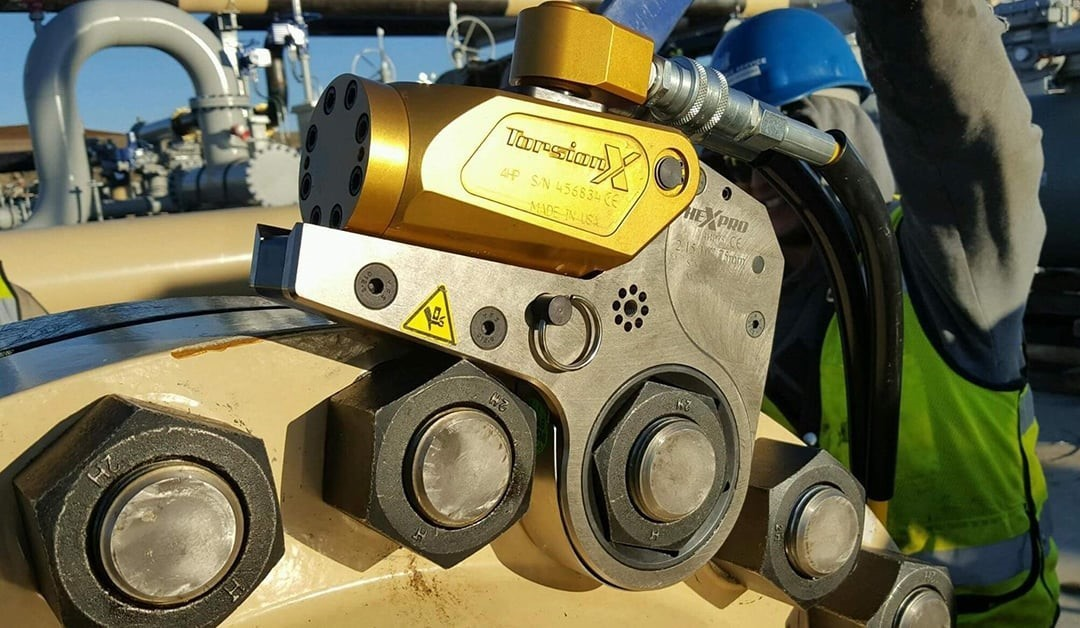
\includegraphics[width= 1\linewidth]{24}
		\caption{\small\textit{\color{toanhocdoisong}Hình $14$. Thiết kế mẫu bom nước cùng các trạng thái mở và gấp lại của nó trong chuyển động.}}
		\vspace*{-5pt}
	\end{figure}
	\begin{figure}[H]
		%		\vspace*{5pt}
		\centering
		\captionsetup{labelformat= empty, justification=centering}
		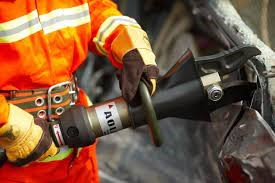
\includegraphics[width= 0.8\linewidth]{25}
		\caption{\small\textit{\color{toanhocdoisong}Hình $15$. Một dạng chuyển động khác của thiết kế bom nước. Sau khi đã gấp và trải phẳng, nếu ta tác động một đầu như trong hình, cấu trúc sẽ uốn lại và sẽ đảo chiều quay trong quá trình chuyển~động.}}
		\vspace*{-10pt}
	\end{figure}
	\begin{figure}[H]
		\vspace*{-10pt}
		\centering
		\captionsetup{labelformat= empty, justification=centering}
		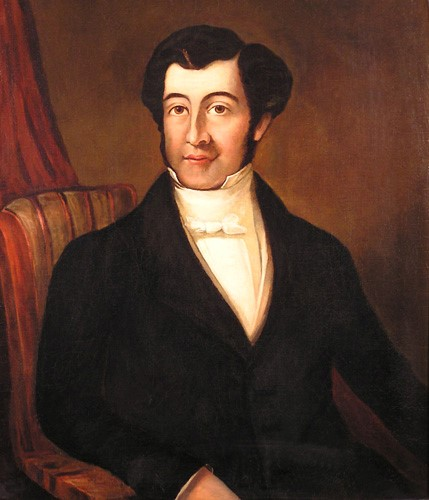
\includegraphics[width= 1\linewidth]{26}
		\caption{\small\textit{\color{toanhocdoisong}Hình $16$. Stent động mạch của You và Kuribayashi--Shigetomi dựa trên thiết kế bom nước. Khi đưa vào cơ thể nó sẽ ở dạng thu gọn, còn khi đến vị trí cần đặt, nó có thể được mở ra thành dạng hoàn chỉnh.}}
		\vspace*{-10pt}
	\end{figure}
	\begin{figure}[H]
		\vspace*{-10pt}
		\centering
		\captionsetup{labelformat= empty, justification=centering}
		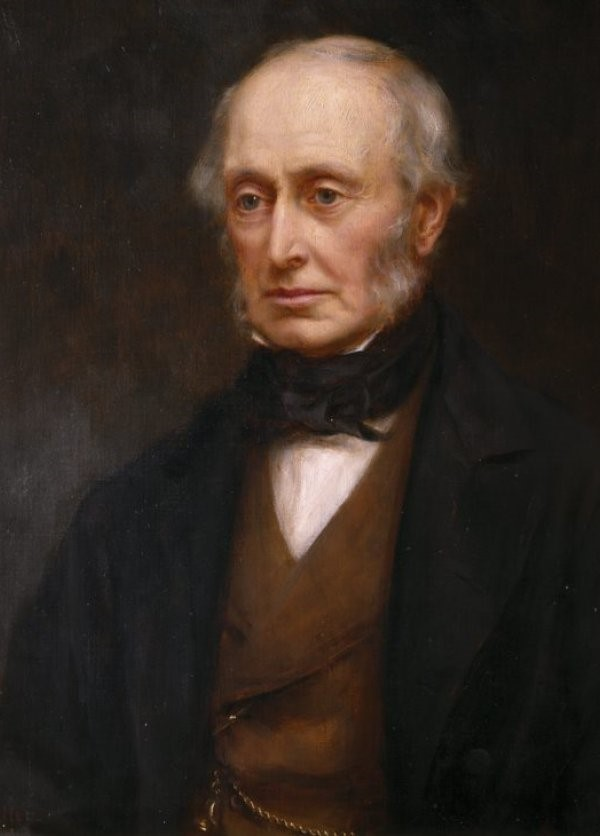
\includegraphics[width= 1\linewidth]{27}
		
		\vspace*{4pt}
		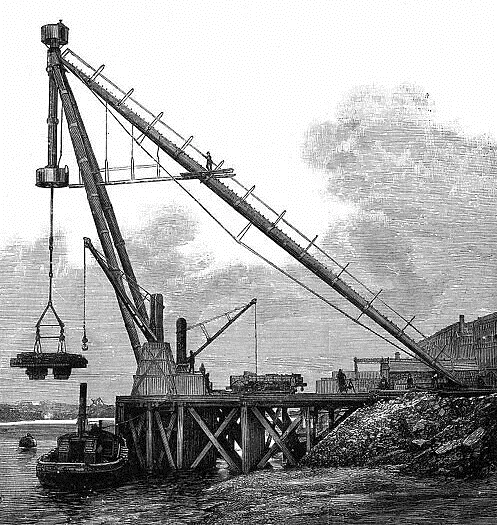
\includegraphics[width= 1\linewidth]{28}
		\caption{\small\textit{\color{toanhocdoisong}Hình $17$. ``Quả bóng kì diệu" của Yuri Shumakov dựa trên thiết kế bomb nước với Miura--ori ở phần biên. Nó có thể có các trạng thái khác nhau khi bị tác động theo phương thẳng đứng.}}
		\vspace*{-5pt}
	\end{figure}
	Còn rất nhiều cách gấp độc đáo khác trong origami hình học mà bạn đọc có thể tìm hiểu trong các tài liệu tham khảo. Trong phần tiếp theo của bài viết, chúng ta sẽ đi sâu hơn về khía cạnh  toán học của origami hình học với nhiều chứng minh thú vị.
	\vskip 0.1cm
	\textbf{\color{toanhocdoisong}Tài liệu tham khảo}
	\vskip 0.1cm
	[$1$]~Felton, S., Tolley, M., Demaine, E., Rus, D., \& Wood, R. ($2014$, Aug). Applied origami. A method for building self--folding machines. \textit{Science}, $644-6$.
	\vskip 0.1cm
	[$2$]~Ginepro, J., \& Hull, T. C. ($2014$). Counting Miura--ori Foldings. \textit{Journal of Integer Sequences}, $17$.
	\vskip 0.1cm
	[$3$]~Hull, T. ($2003$). Counting Mountain--Valley Assignments for Flat Folds. \textit{Ars Combinatoria}, $67$, $175-188$.
	\vskip 0.1cm
	[$4$]~Lang, R. J. ($2009$). \textit{Origami$4$}. AK Peters.
	\vskip 0.1cm
	[$5$]~Lang, R. J. ($2018$). \textit{Twists, Tilings, and Tessellations. Mathematical Methods for Geometric Origami}. CRC Press.
	\vskip 0.1cm
	[$5$] Tachi, T., \& Hull, T. C. ($2017$, April). Self--Foldability of Rigid Origami. \textit{Journal of Mechanisms and Robotics}, $9$.
\end{multicols}
